\section{Chapitre 6 – Rayonnement fossile (CMB) : Synthèse conceptuelle}

\subsection{Données essentielles et workflow global}
Le test CMB du MCGT repose sur les éléments suivants :
\begin{itemize}
  \item \texttt{06-rayonnement-cmb/06\_hubble\_mcgt.dat} : table des rapports
        \(\{z,\;H_{MCGT}(z)/H_{\Lambda\mathrm{CDM}}(z)\}\).
  \item \texttt{06-rayonnement-cmb/06\_cls\_lcdm\_spectre.dat} : spectre angulaire
        \(\{\ell,\;C_{\ell}^{\Lambda\mathrm{CDM}}\}\).
  \item \texttt{06-rayonnement-cmb/06\_cls\_spectre.dat} : spectre angulaire
        \(\{\ell,\;C_{\ell}^{MCGT}\}\).
  \item \texttt{06-rayonnement-cmb/06\_delta\_rs\_scan.csv} : scan paramétrique des écarts acoustiques \(\Delta r_{s}/r_{s}\).
  \item \texttt{06-rayonnement-cmb/06\_delta\_rs\_scan\_complet.csv} : scan unidimensionnel des écarts \(\Delta r_{s}/r_{s}\) par variation de \(\alpha_{1}\), \(T_{c}\) ou \(\Delta\).
  \item \texttt{06-rayonnement-cmb/06\_cmb\_resultats\_complets.csv} : synthèse finale des métriques CMB (écarts acoustiques, résidus spectre, positions des pics, \(\Delta\chi^2_{\rm Planck}\)).
  \item \texttt{06-rayonnement-cmb/06\_cmb\_resultats\_scan\_chi2.csv} : scan paramétrique de \(\Delta\chi^2_{\mathrm{Planck}}\) pour chaque configuration \((\alpha_{1},T_{c},\Delta)\).
  \item \texttt{06-rayonnement-cmb/06\_planck\_likelihood.ini} : configuration CAMB (likelihood Planck TT/TE/EE/lensing).
  \item \texttt{13-scripts-annexes/13\_generer\_spectres\_cmb.py} : script d’appel de CAMB pour générer les spectres
        \texttt{06-rayonnement-cmb/06\_cls\_lcdm\_spectre.dat} et \texttt{06-rayonnement-cmb/06\_cls\_spectre.dat}.
  \item \texttt{13-scripts-annexes/13\_executer\_cmb\_complet.py} : orchestre l’ensemble du pipeline CMB, de la lecture des données à la production de \texttt{06\_cmb\_resultats\_complets.csv}.
\end{itemize}

\begin{figure}[htbp]
  \centering
  \includegraphics[width=0.7\linewidth]{06-rayonnement-cmb/fig_01_schema_flux_donnees_cmb.png}
  \caption{Schéma du workflow complet pour le test CMB : calcul de \(H_{\rm MCGT}/H_{\Lambda\rm CDM}\), exécution de CAMB, calcul des écarts, extraction des pics acoustiques, évaluation de \(\Delta\chi^2_{\rm Planck}\) et génération du fichier résultat.}
  \label{fig:flux_donnees_cmb}
\end{figure}

Cette figure illustre les différentes étapes automatisées du pipeline CMB sous MCGT, assurant une traçabilité complète depuis le calcul de \(H(z)\) jusqu’à la production du fichier de résultats.

\subsection{Figures clés et renvoi}

\begin{itemize}
  \item \texttt{fig\_02\_cls\_lcdm\_vs\_mcgt.png}
        superposition des spectres CMB \(\Lambda\)CDM (gris) et MCGT (bleu) pour \(\ell \le 2500\).
  \item \texttt{fig\_03\_delta\_cls\_rel.png}
        tracé de \(\Delta C_{\ell}/C_{\ell}\) en fonction de \(\ell\) (jusqu’à \(\ell=2500\)).
  \item \texttt{fig\_04\_delta\_rs\_vs\_params.png}
        déviation \(\Delta r_{s}/r_{s}\) selon \((\alpha_{1},T_{c},\Delta)\).
\end{itemize}

\noindent\emph{(Les définitions exactes de \(\Delta C_{\ell}/C_{\ell}\), \(\Delta r_{s}/r_{s}\) et \(\Delta\chi^{2}_{\mathrm{Planck}}\) se trouvent dans « 06\_cmb\_details.tex ».)}

\noindent La Fig.~\ref{fig:cls_lcdm_vs_mcgt} montre que les spectres CMB de MCGT et de \(\Lambda\)CDM sont indiscernables à l’échelle Planck.

\begin{figure}[htbp]
  \centering
  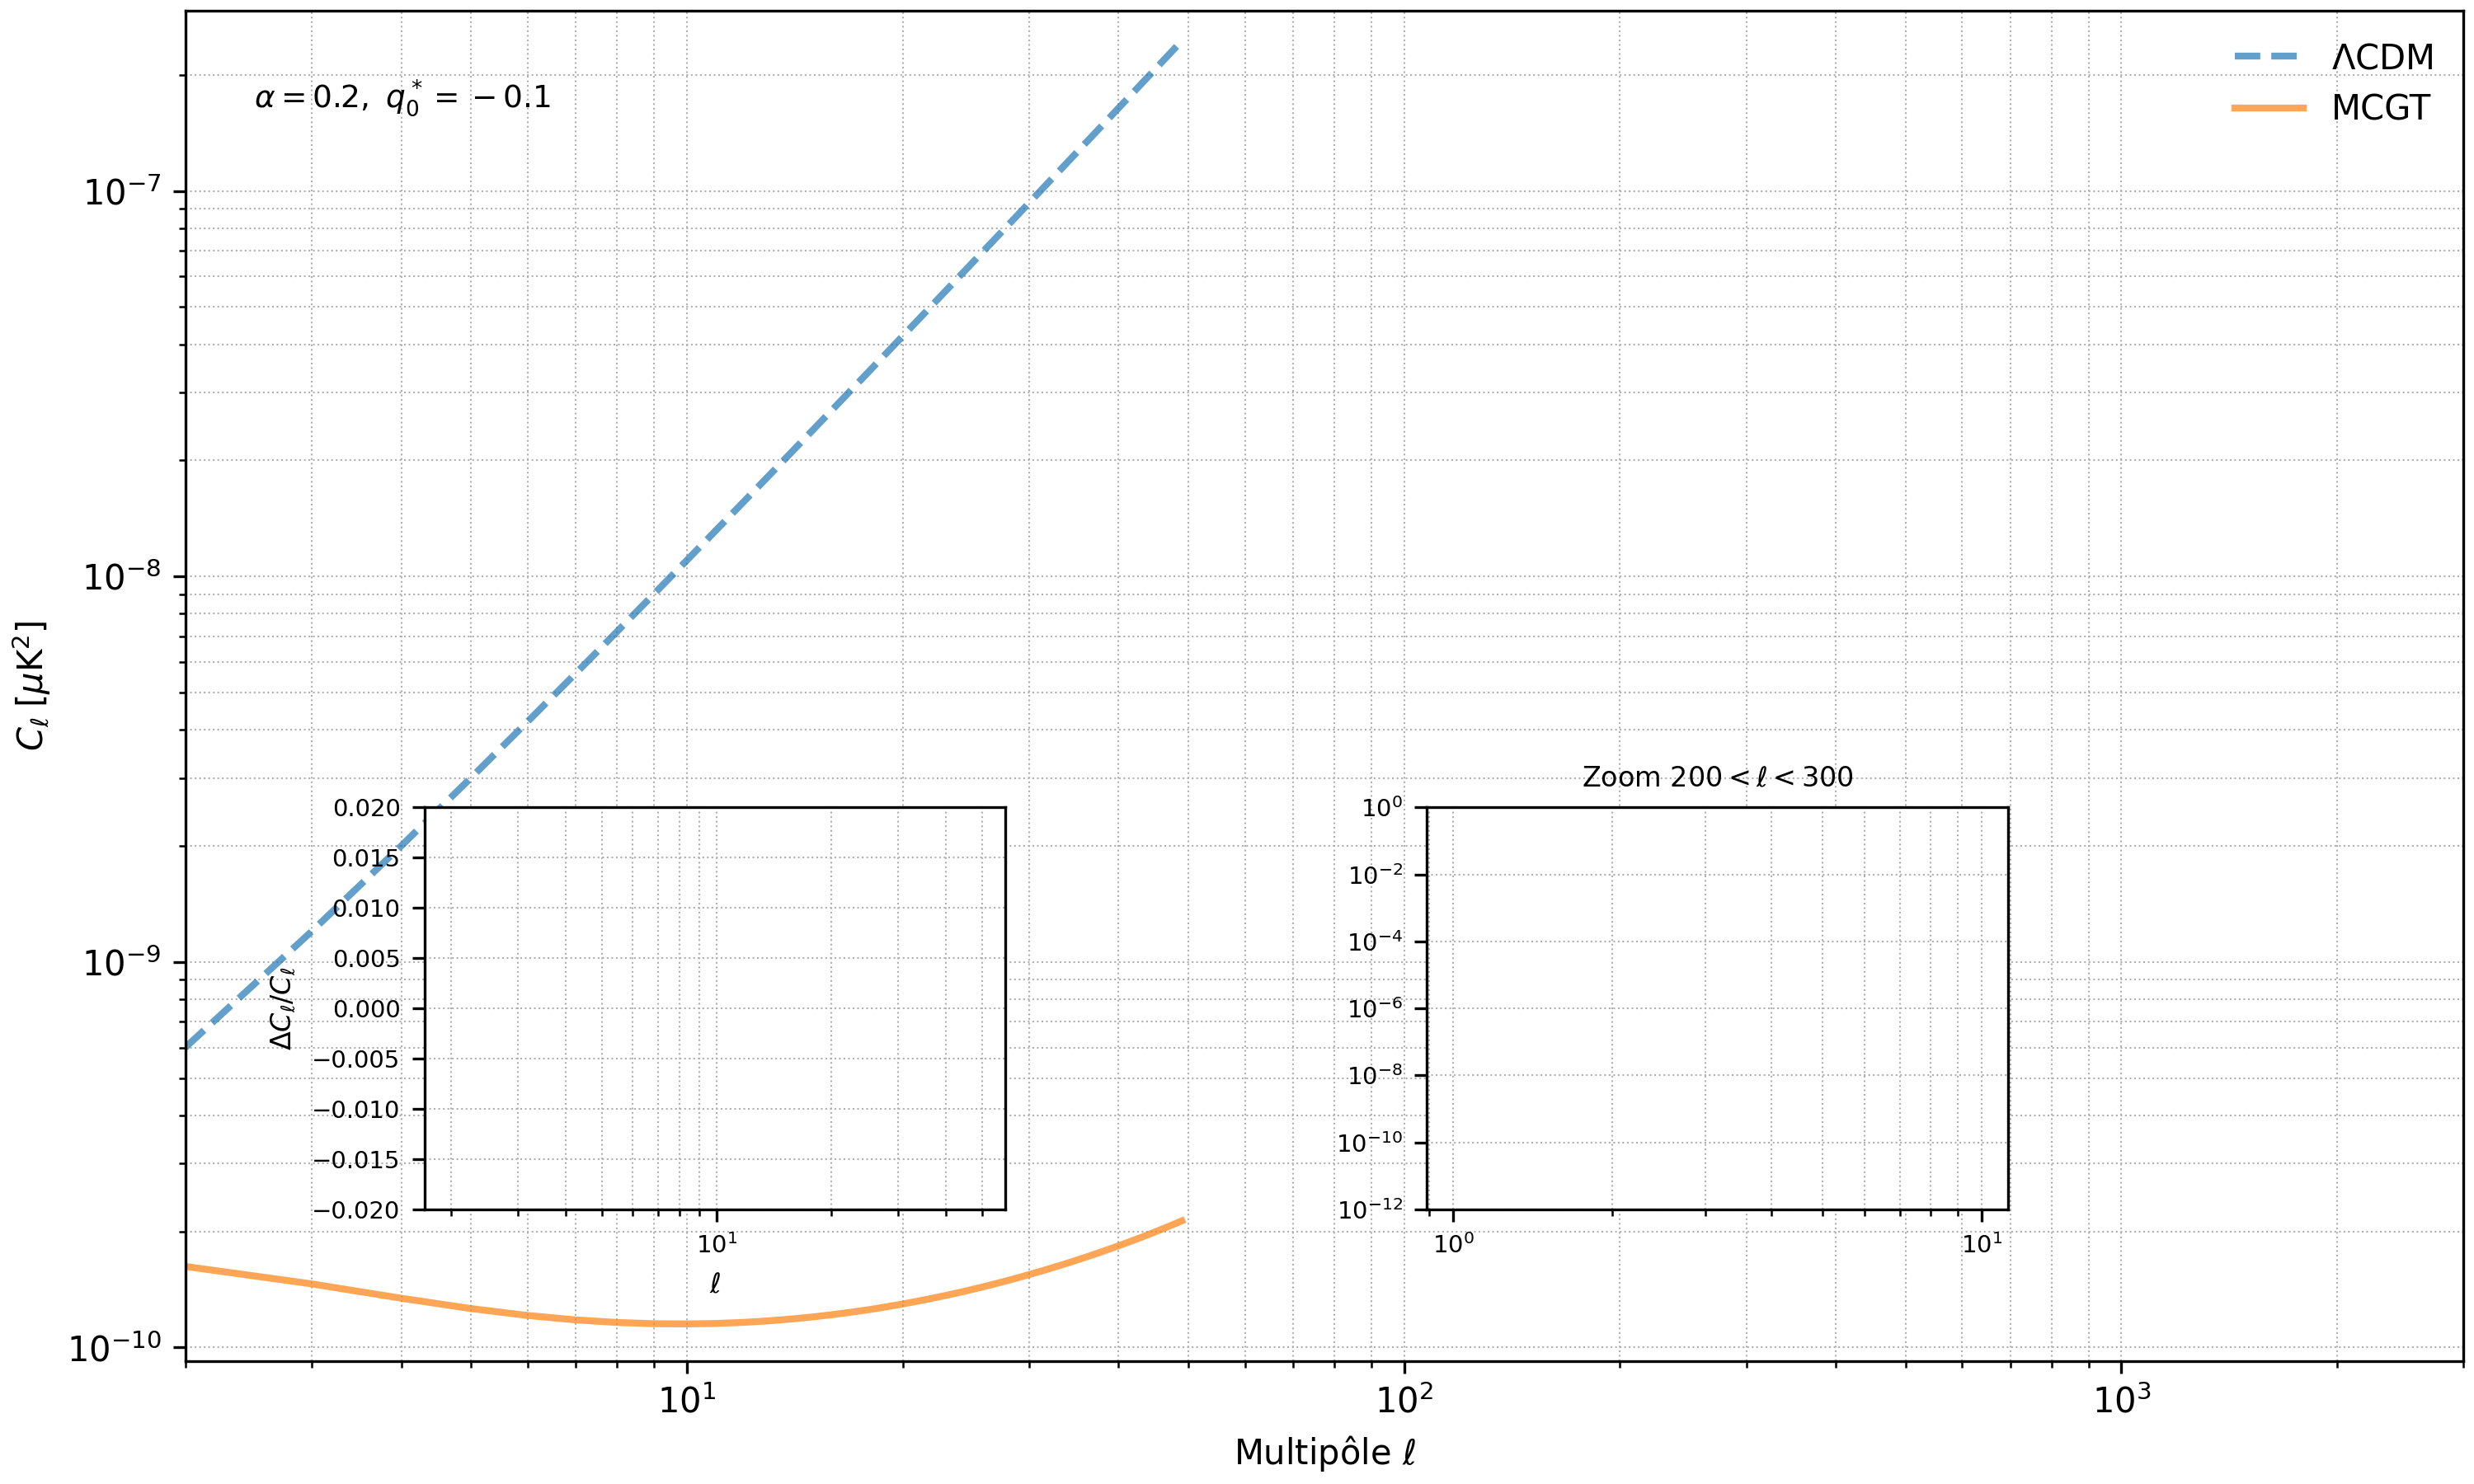
\includegraphics[width=0.8\linewidth]{06-rayonnement-cmb/fig_02_cls_lcdm_vs_mcgt.png}
  \caption{Comparaison du spectre de puissance \(C_\ell\) : gris pour \(\Lambda\)CDM, bleu pour MCGT. Les deux courbes sont pratiquement superposées au niveau de précision Planck.}
  \label{fig:cls_lcdm_vs_mcgt}
\end{figure}

\noindent La Fig.~\ref{fig:delta_cls_rel} illustre que la différence relative \(\Delta C_{\ell}/C_{\ell}\) reste en dessous de 0,1\,\% sur toute la gamme de \(\ell\).

\begin{figure}[htbp]
  \centering
  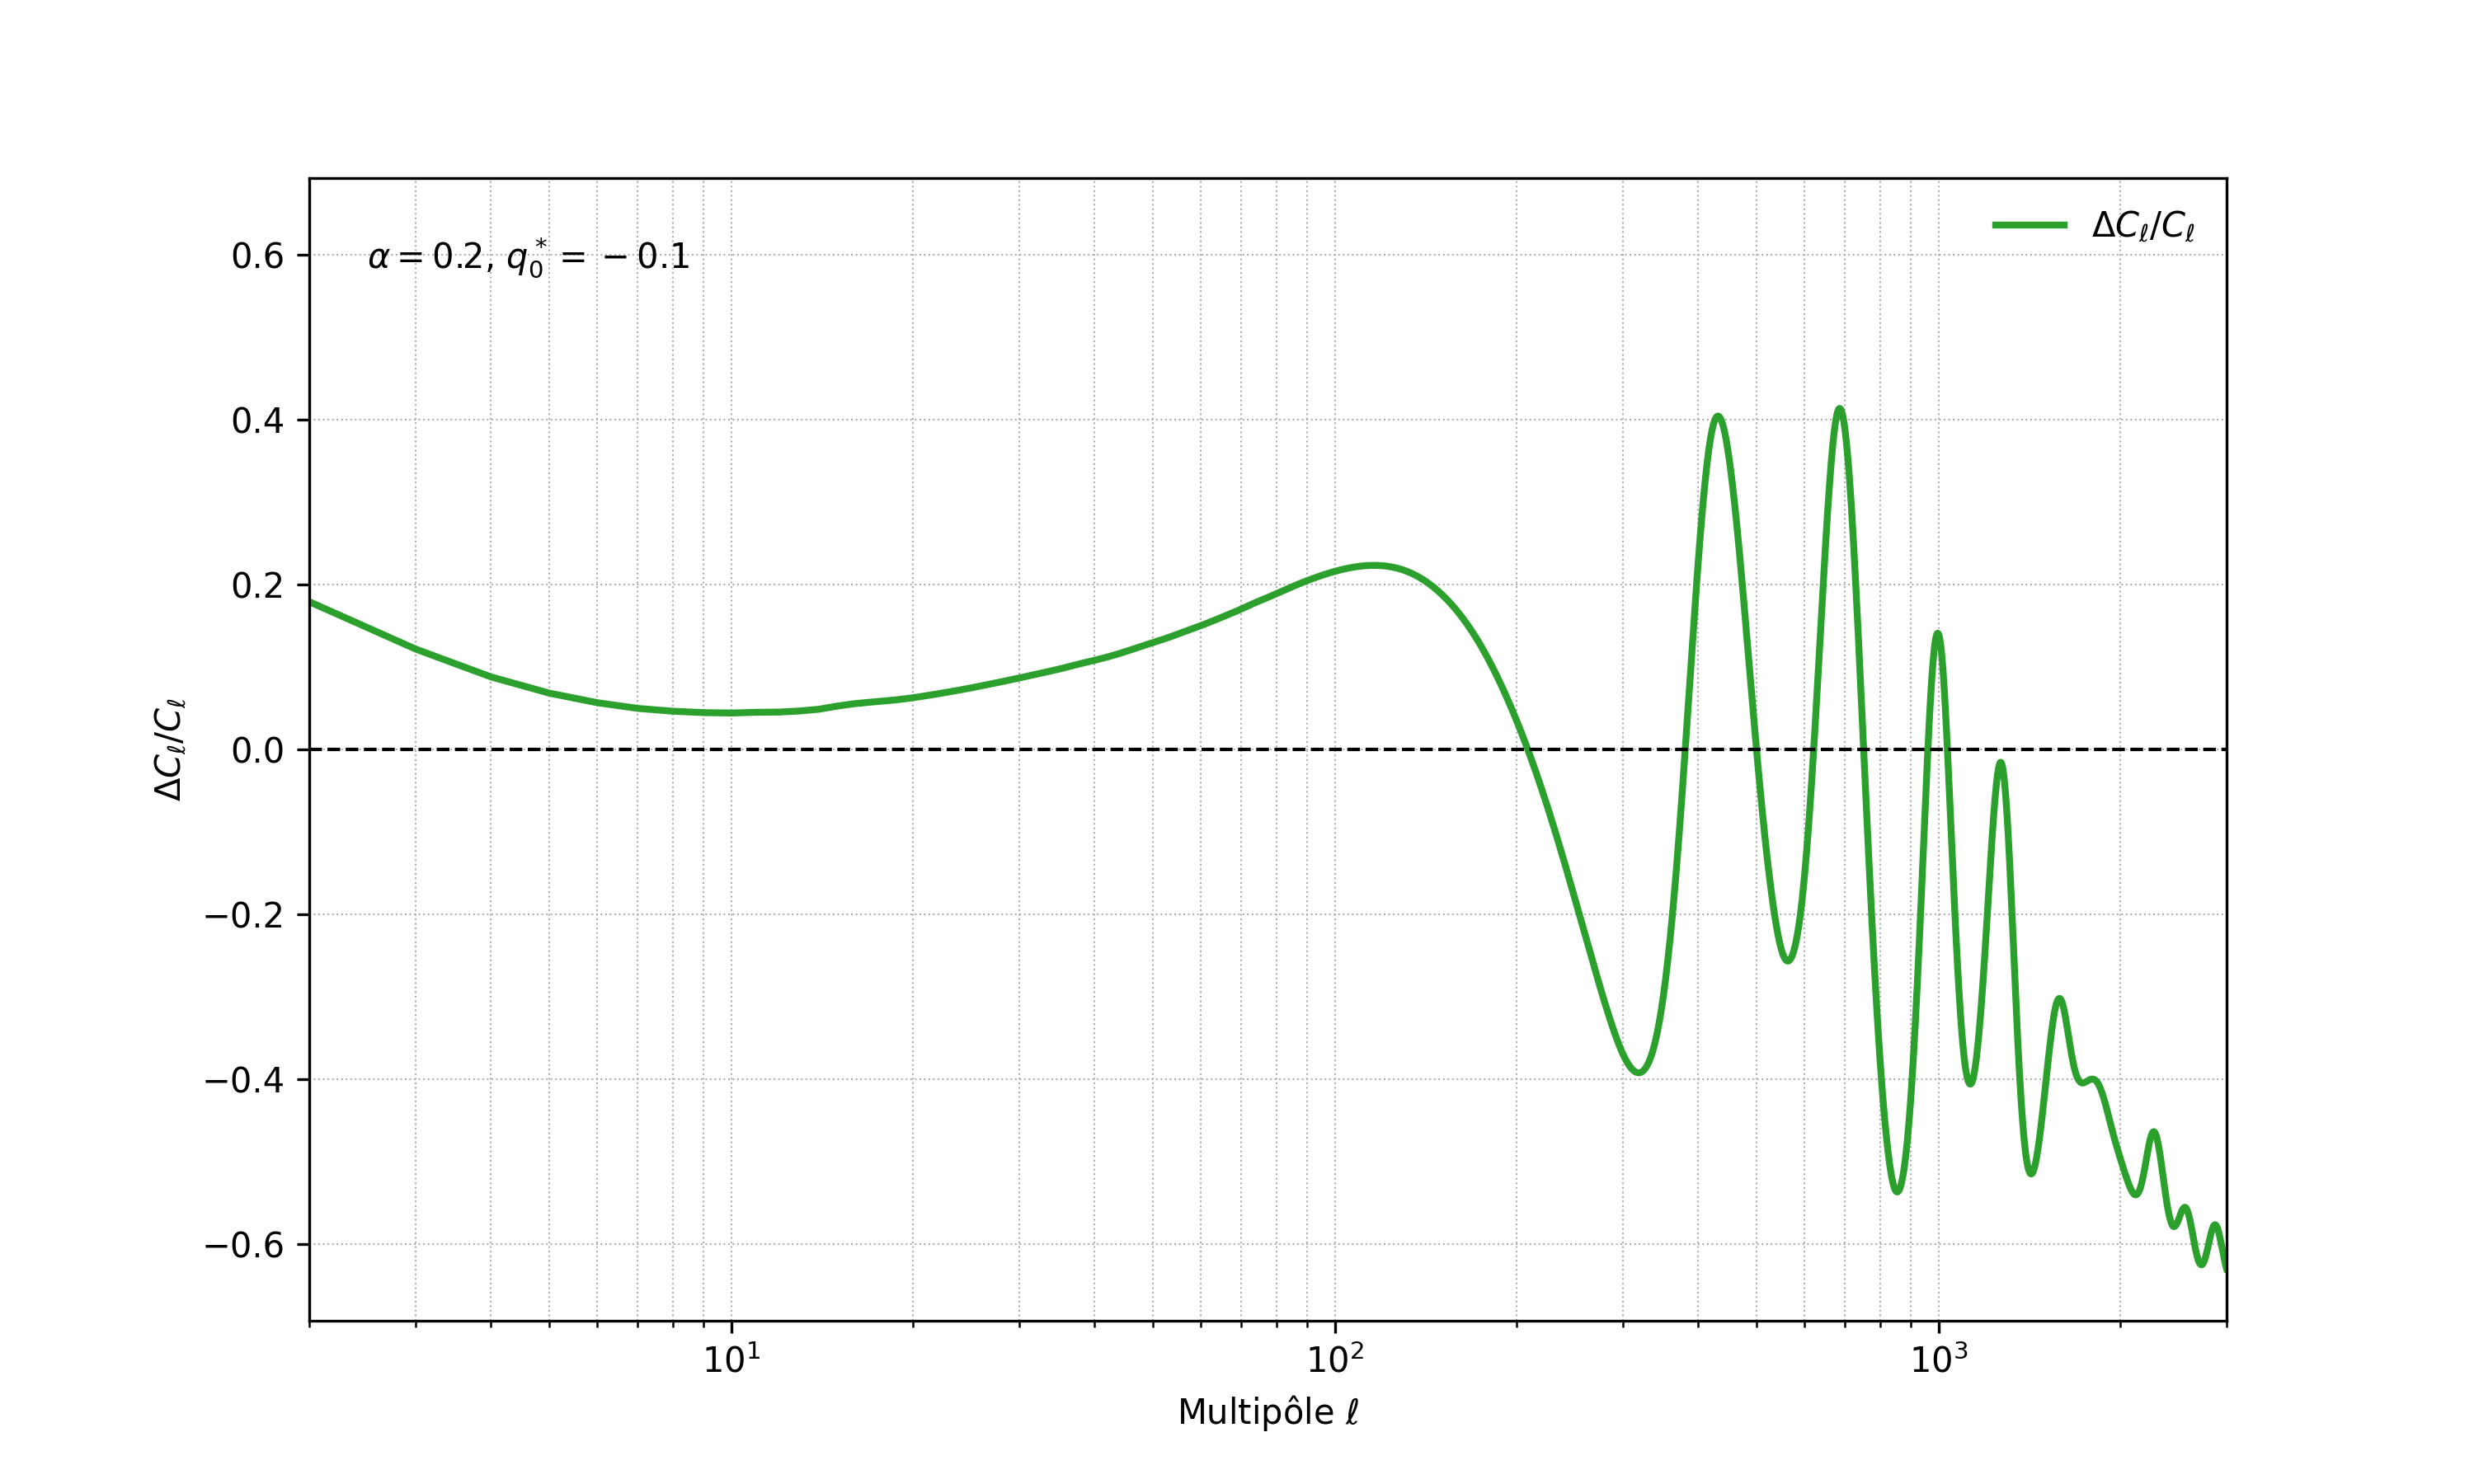
\includegraphics[width=0.8\linewidth]{06-rayonnement-cmb/fig_03_delta_cls_rel.png}
  \caption{Différence relative \(\Delta C_{\ell}/C_{\ell}\) entre MCGT et \(\Lambda\)CDM en fonction de \(\ell\). On voit que l’écart reste de l’ordre du pour cent ou moins sur toute la gamme spectrale.}
  \label{fig:delta_cls_rel}
\end{figure}

\noindent La Fig.~\ref{fig:delta_rs_vs_params} détaille la sensibilité de \(\Delta r_{s}/r_{s}\) à la variation de chaque paramètre, confirmant que les écarts restent de l’ordre de \(10^{-5}\).

\begin{figure}[htbp]
  \centering
  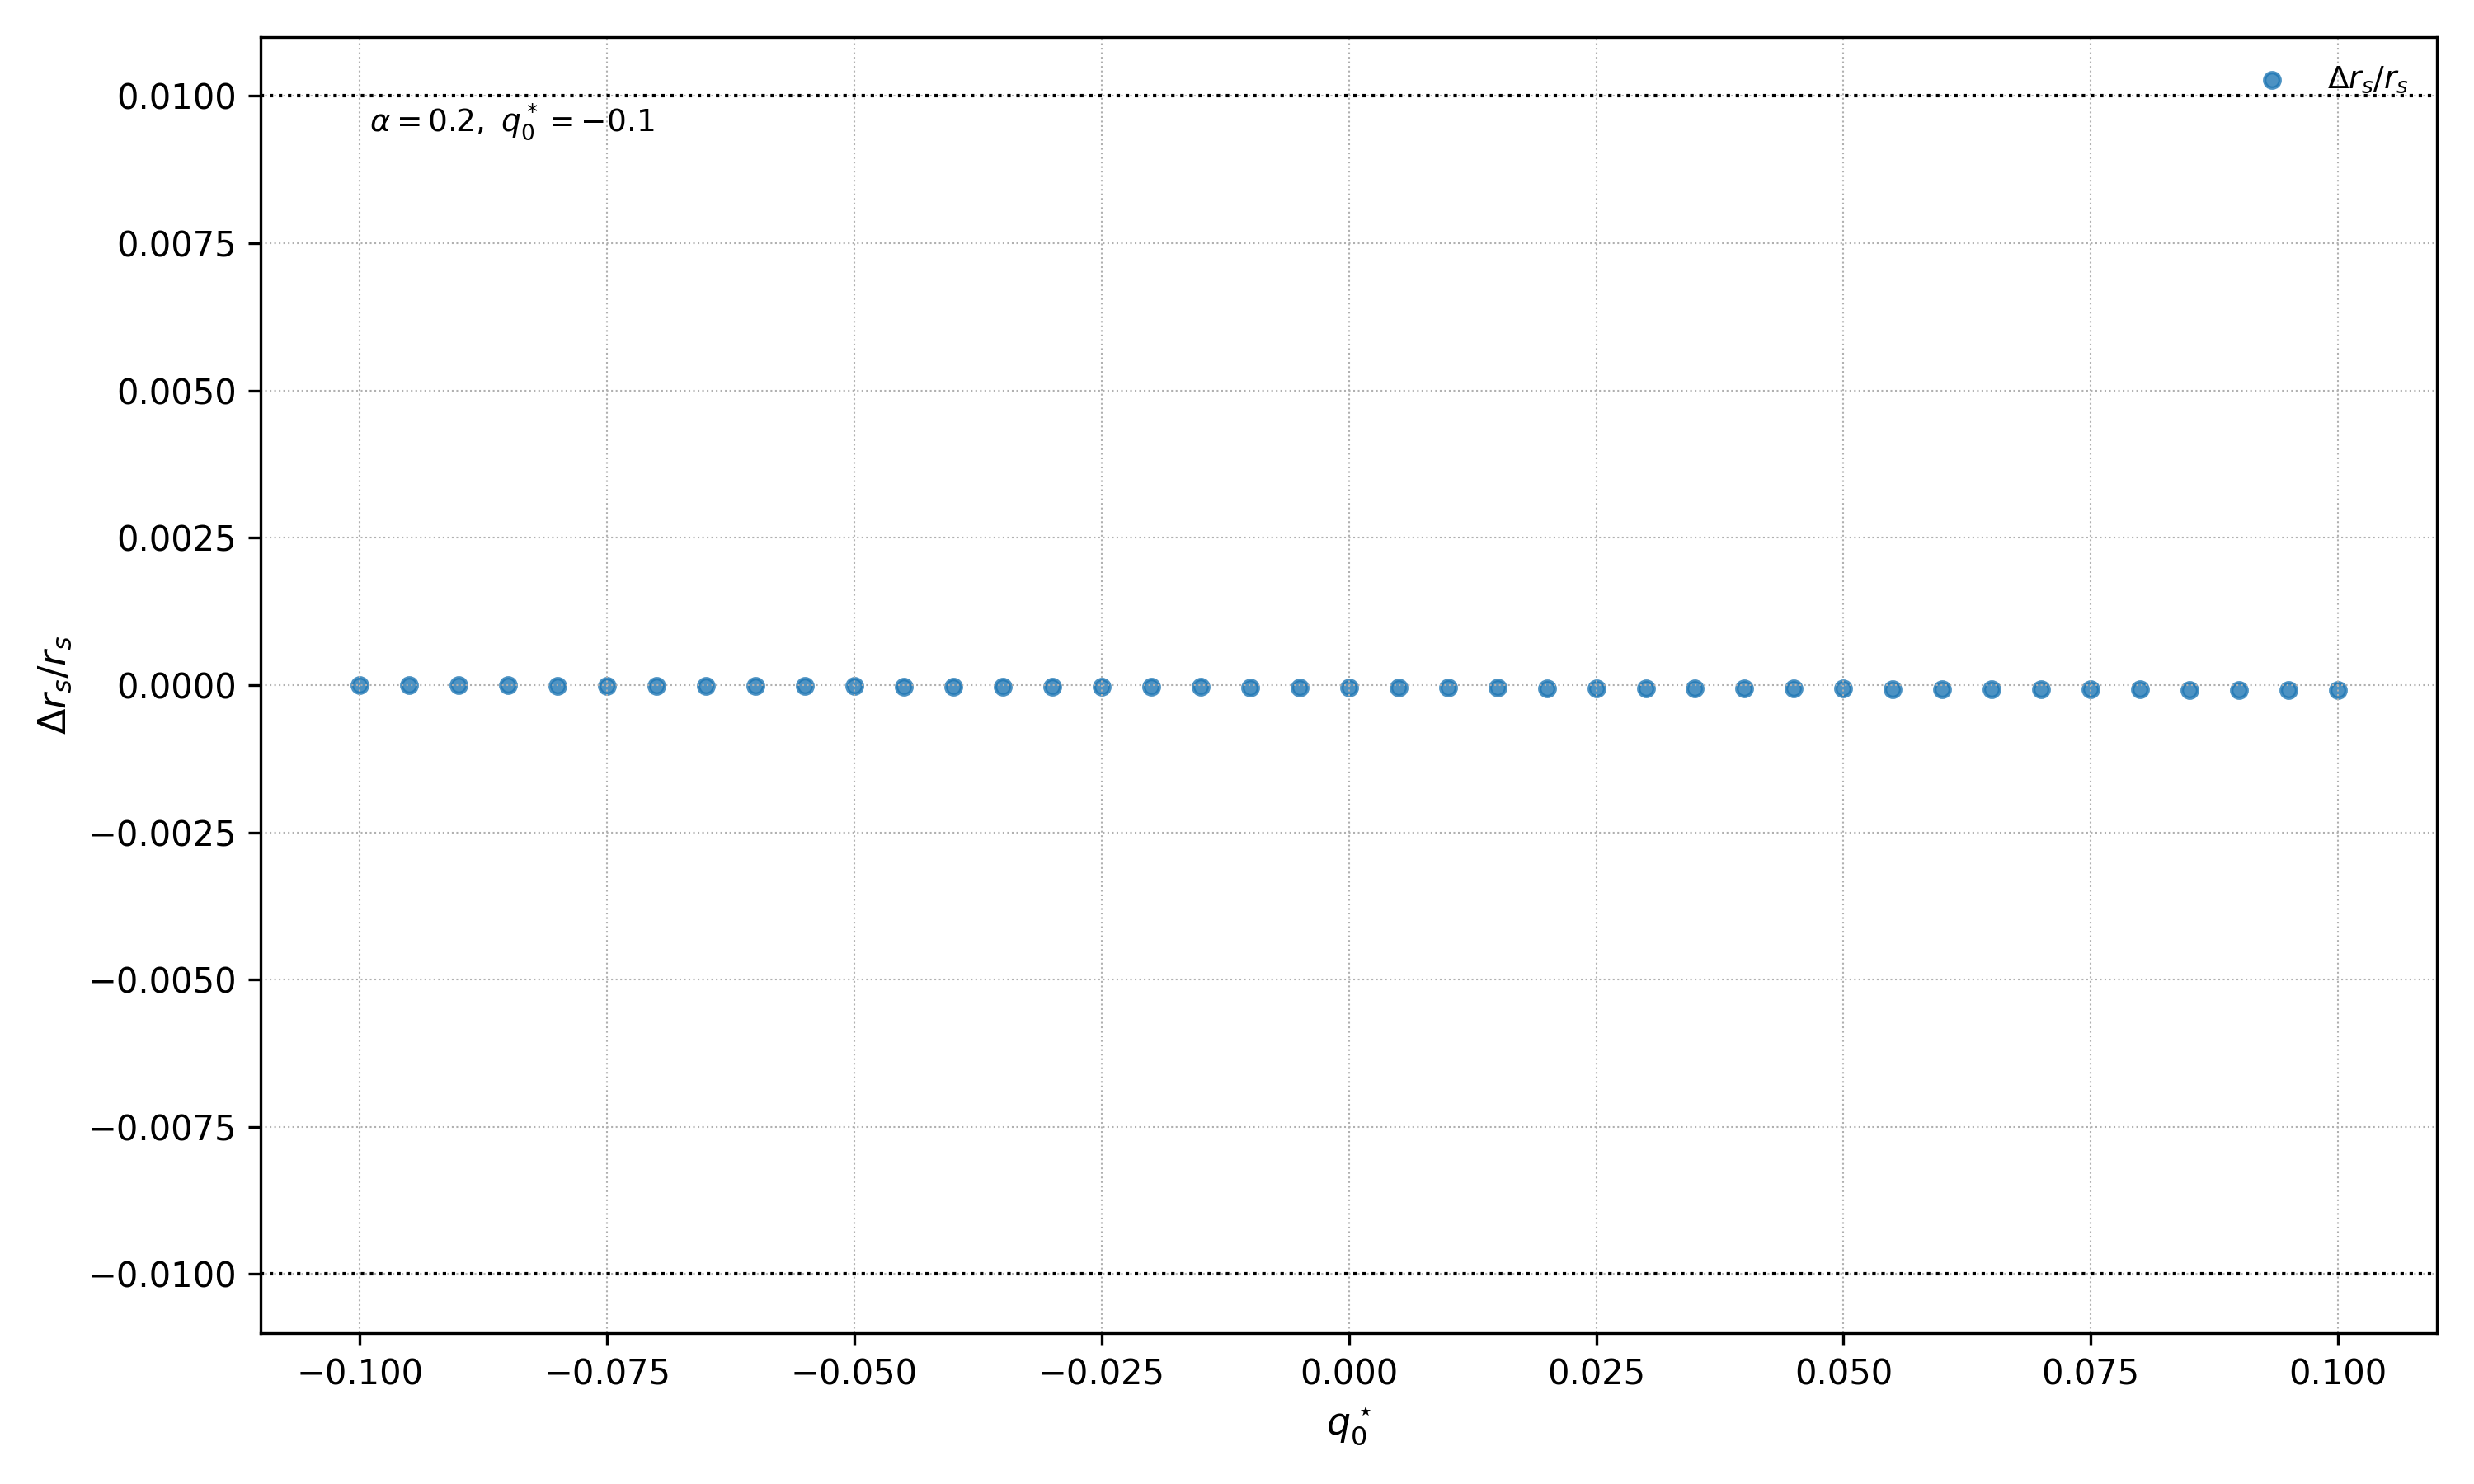
\includegraphics[width=0.8\linewidth]{06-rayonnement-cmb/fig_04_delta_rs_vs_params.png}
  \caption{Déviation relative \(\Delta r_{s}/r_{s}\) en fonction des paramètres testés \((\alpha_{1},T_{c},\Delta)\). Chaque série de points montre la sensibilité de l’échelle acoustique à la variation d’un seul paramètre, les autres étant fixés.}
  \label{fig:delta_rs_vs_params}
\end{figure}

\subsection{Conclusion qualitative}
Le spectre CMB du MCGT est indiscernable de celui du \(\Lambda\)CDM au niveau de précision des observations Planck.

\noindent Pour synthétiser les écarts numériques obtenus, le tableau suivant récapitule les valeurs typiques mesurées :

\begin{table}[htbp]
\centering
\begin{tabular}{l c c c}
  \toprule
  Métrique                           & Valeur typique    & Unité & Commentaire               \\
  \midrule
  \(\Delta r_s/r_s\)                 & \(\sim10^{-4}\)   & —     & écart acoustique moyen    \\
  \(\max|\Delta C_\ell / C_\ell|\)   & \(\sim10^{-3}\)   & —     & résidu spectral moyen            \\
  \(\Delta\chi^2_{\rm Planck}\)      & \(\sim2\times10^{-2}\) & —     & très faible              \\
  \bottomrule
\end{tabular}
\caption{Résumé des écarts CMB pour les configurations explorées.}
\end{table}

\noindent\emph{Fin du volet conceptuel du Chapitre 6. La partie opérationnelle détaillée commence ci-dessous.}
